\documentclass[a4paper]{article}
\usepackage[utf8x]{inputenc}
\usepackage[T1,T2A]{fontenc}
\usepackage[russian]{babel}
\usepackage{hyperref}
\usepackage{indentfirst}
\usepackage{listings}
\usepackage{color}
\usepackage{here}
\usepackage{array}
\usepackage{multirow}
\usepackage{graphicx}
\usepackage{caption}
\graphicspath{{graphics/}}
\usepackage[left=2cm,right=2cm,
top=2cm,bottom=2cm,bindingoffset=0cm]{geometry}
\usepackage{listings}
\lstset{ %
	extendedchars=\true,
	keepspaces=true,
	language=bash,					% choose the language of the code
	basicstyle=\footnotesize,		% the size of the fonts that are used for the code
	numbers=left,					% where to put the line-numbers
	numberstyle=\footnotesize,		% the size of the fonts that are used for the line-numbers
	stepnumber=1,					% the step between two line-numbers. If it is 1 each line will be numbered
	numbersep=5pt,					% how far the line-numbers are from the code
	backgroundcolor=\color{white},	% choose the background color. You must add \usepackage{color}
	showspaces=false				% show spaces adding particular underscores
	showstringspaces=false,			% underline spaces within strings
	showtabs=false,			 		% show tabs within strings adding particular underscores
	frame=single,           		% adds a frame around the code
	tabsize=2,						% sets default tabsize to 2 spaces
	captionpos=b,					% sets the caption-position to bottom
	breaklines=true,				% sets automatic line breaking
	breakatwhitespace=false,		% sets if automatic breaks should only happen at whitespace
	escapeinside={\%*}{*)},			% if you want to add a comment within your code
	postbreak=\raisebox{0ex}[0ex][0ex]{\ensuremath{\color{red}\hookrightarrow\space}}
}

\begin{document}	% начало документа

\begin{titlepage}	% начало титульной страницы

	\begin{center}		% выравнивание по центру

		\large Санкт-Петербургский Политехнический Университет Петра Великого\\
		\large Институт компьютерных наук и технологий \\
		\large Кафедра компьютерных систем и программных технологий\\[6cm]
		% название института, затем отступ 6см
		
		\huge Телекоммуникационные технологии\\[0.5cm] % название работы, затем отступ 0,5см
		\large Отчет по лабораторной работе №1 \\[0.1cm]
		\large\textbf{"Сигналы телекоммуникационных систем"}\\[5cm]

	\end{center}


	\begin{flushright} % выравнивание по правому краю
		\begin{minipage}{0.25\textwidth} % врезка в половину ширины текста
			\begin{flushleft} % выровнять её содержимое по левому краю

				\large\textbf{Работу выполнил:}\\
				\large Курякин Д. А.\\
				\large {Группа:} 33501/4\\
				
				\large \textbf{Преподаватель:}\\
				\large Богач Н.В.\

			\end{flushleft}
		\end{minipage}
	\end{flushright}
	
	\vfill % заполнить всё доступное ниже пространство

	\begin{center}
	\large Санкт-Петербург\\
	\large \the\year % вывести дату
	\end{center} % закончить выравнивание по центру

\thispagestyle{empty} % не нумеровать страницу
\end{titlepage} % конец титульной страницы

\vfill % заполнить всё доступное ниже пространство

\section{Цель работы}
Познакомиться со средствами генерации и визуализации простых сигналов.

\section{Постановка задачи}
В командном окне MATLAB и в среде Simulink промоделировать синусоидальный и прямоугольный сигналы с различными параметрами. Получить их спектры. Вывести на график.

\section{Теоретический раздел}
\subsection{Сигнал}
{\bfseries Сигнал} — изменение физической величины, несущее информацию, кодированную определённым способом. Сигналом может быть любой физический процесс, параметры которого изменяются (или находятся) в соответствии с передаваемым сообщением.

 {\bfseries Класификация сигналов}
\begin{itemize}
	\itemДетерминированный сигнал - это  сигнал, характеристики которого могут быть определены в любой момент времени с вероятностью равной единице. Детерминированные сигралы делятся на на  \textit{периодические} и \textit{непиреодические} сигналы. К периодическим относят гармонические и полигармонические сигналы. Для периодических сигналов выполняется общее условие 
	\begin{equation}
	s(t) = s(t + kT),
	\end{equation}
	где k = 1, 2, 3, ... - любое целое число, Т - период, являющийся конечным отрезком независимой переменной.
	\itemСлучайный сигнал - это такой сигнал, значение которых в любой момент времени невозможно предсказать с вероятностью равной единице.
\end{itemize}

{\bfseries Аналоговый сигнал} - это сигнал, у которого каждый из представляющих параметров описывается функцией времени и непрерывным множеством возможных значений. Большинство сигналов имеют аналоговую природу, то есть изменяются непрерывно во времени и могут принимать любые значения на некотором интервале. Аналоговые сигналы описываются некоторой математической функцией времени.

{\bfseries Дискретный сигнал} представляется в виде последовательности значений, взятых в дискретные моменты времени. Обычно промежутки времени между последовательными отсчётами постоянны.

\subsection{Преобразование Фурье}
{\bfseries Преобразование Фурье} - это операция, сопоставляющая одной функции вещественной переменной другую функцию вещественной переменной. Преобразования Фурье осуществляется с помощью ряда Фурье и с помощью интеграла Фурье, причём первый применяется когда функция периодическая, а второй когда она апериодична.

Ряд Фурье — представление функции  f с периодом $\tau$ в виде ряда
\begin{equation}
f(x) = {a_0\over 2} + \sum_{k=1}^{+\infty}A_k cos(k{2\pi\over 
	\tau}x + \theta_k)
\end{equation}

Преобразования Фурье

\begin{equation}
S(\omega) = \int_{-\infty}^{\infty} s(t)e^{-j\omega t} dt.
\end{equation}

Обратное преобразование Фурье

\begin{equation}
s(t) = \frac{1}{2\pi} \int_{-\infty}^{\infty} S(\omega)e^{j\omega t} d\omega.
\end{equation}

\section{Ход работы}
\subsection{Моделирование в Matlab}
\subsubsection{Моделирование синусоидального сигнала}

В командном окне Matlab промоделируем синусоидальные сигналы с разными параметрами и найдем их спектры. 

\begin{center}
	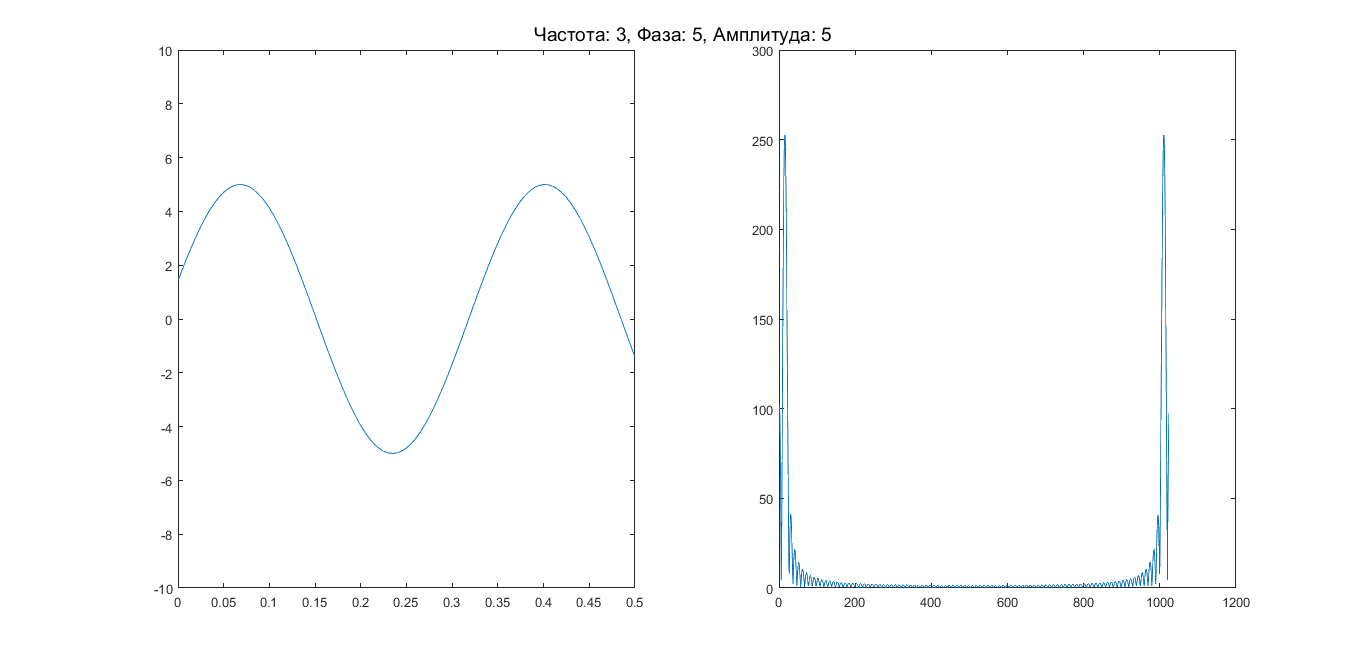
\includegraphics[scale = 0.5]{pictures/s3_5_5.png}
	\\ Рис.1 Синусоидальные сигнал и его спектр
	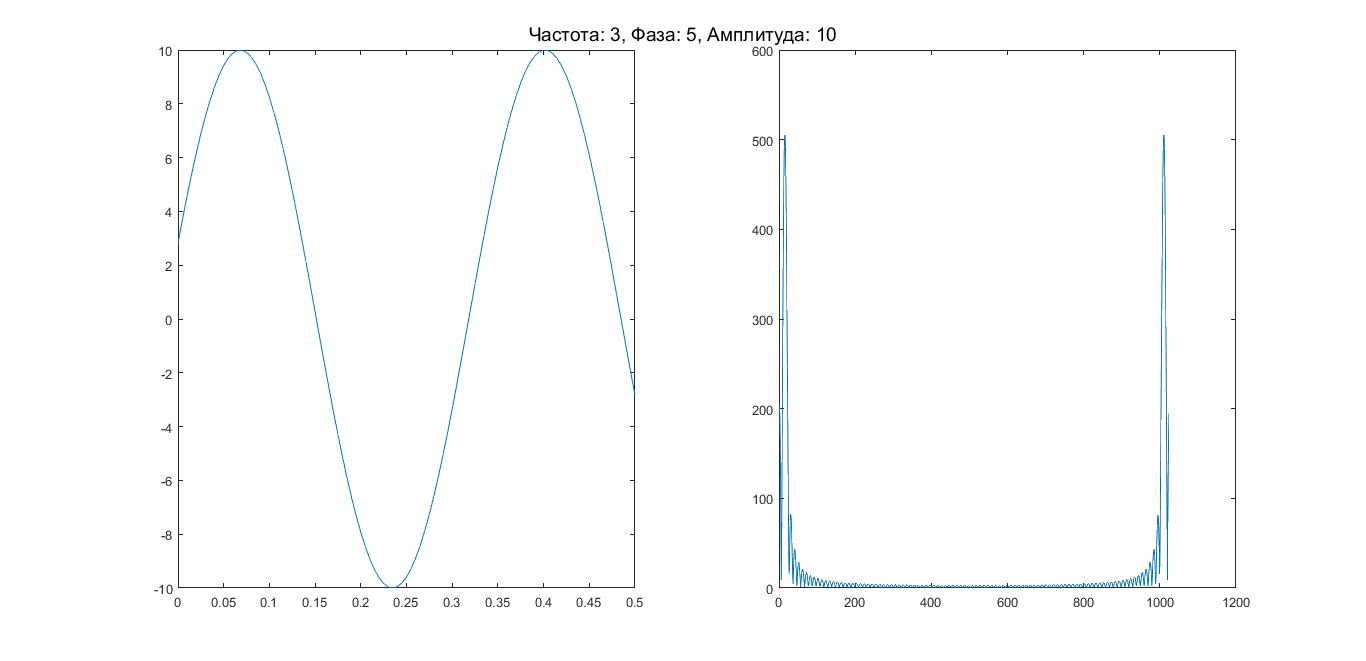
\includegraphics[scale = 0.5]{pictures/s3_5_10.png}
	\\ Рис.2 Синусоидальные сигнал и его спектр
	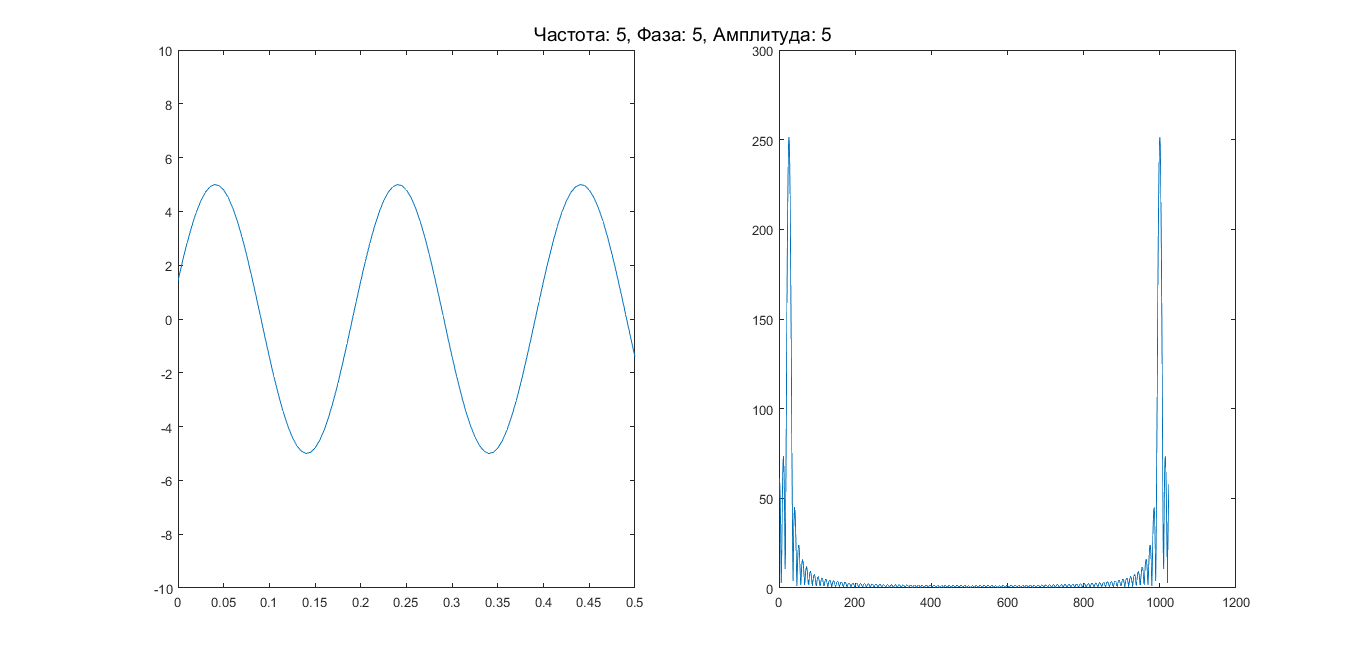
\includegraphics[scale = 0.5]{pictures/s5_5_5.png} 
	\\ Рис.3 Синусоидальные сигнал и его спектр
\end{center} 

В среде Simulink промоделируем синусоидальный сигнал, для этого построим следующую схему.

\begin{center}
	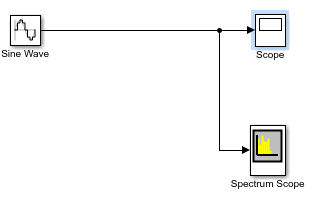
\includegraphics[scale = 0.5]{pictures/sin.png} 
	\\ Рис.4 Схема
\end{center} 
	
В настройках Sin Wave установим:
\begin{verbatim}
	Sine type: Sample based
	Time: Use simulation time
	Amplitude: 1
	Bise: 0
	Samples per period: 100
	Number of offset samples: 0
	Sample time: 0.01
\end{verbatim}

	\center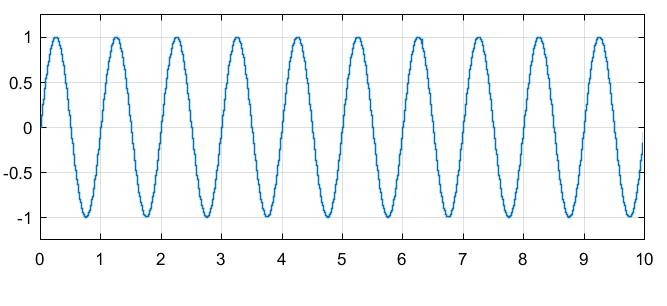
\includegraphics[scale = 0.5]{pictures/S.png} 
	\\ \centerРис.5 Сигнал
	\center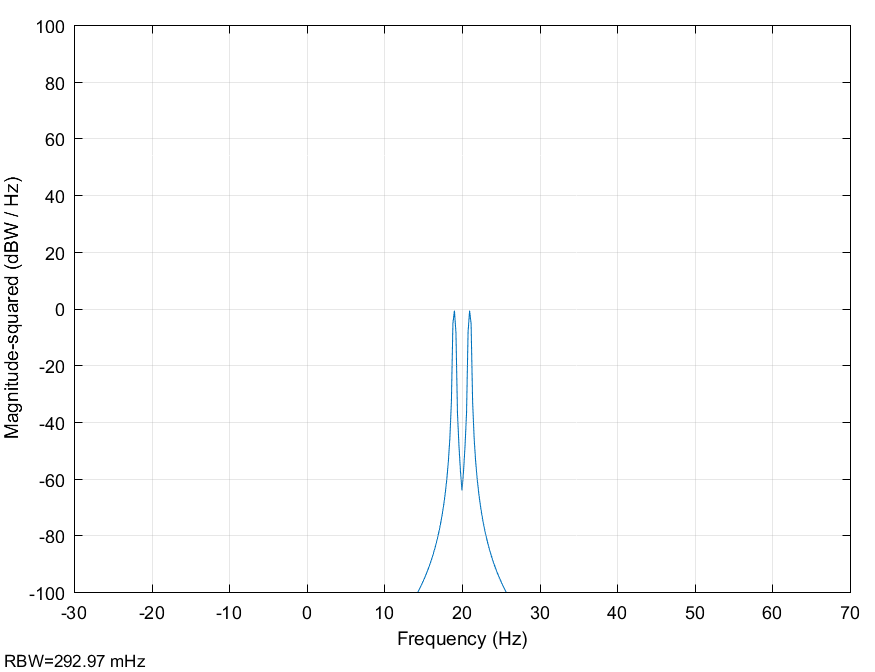
\includegraphics[scale = 0.5]{pictures/ms_S.png} 
	\\ \centerРис.6 Спектр

\newpage

\subsubsection{Моделирование прямоугольного сигнала}
В командном окне Matlab промоделируем прямоугольные сигналы с разными параметрами и найдем их спектры. 


\begin{center}
	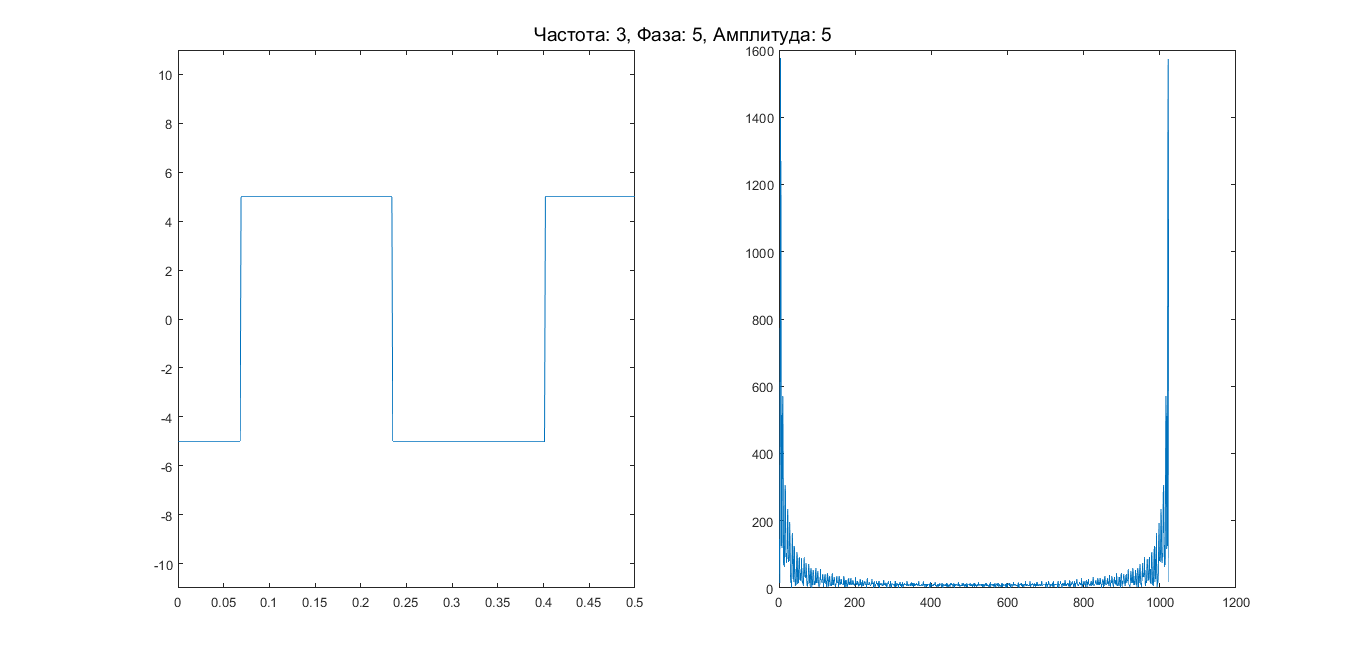
\includegraphics[scale = 0.5]{pictures/3_5_5.png}
	\\ Рис.7 Прямоугольные сигнал и его спектр
	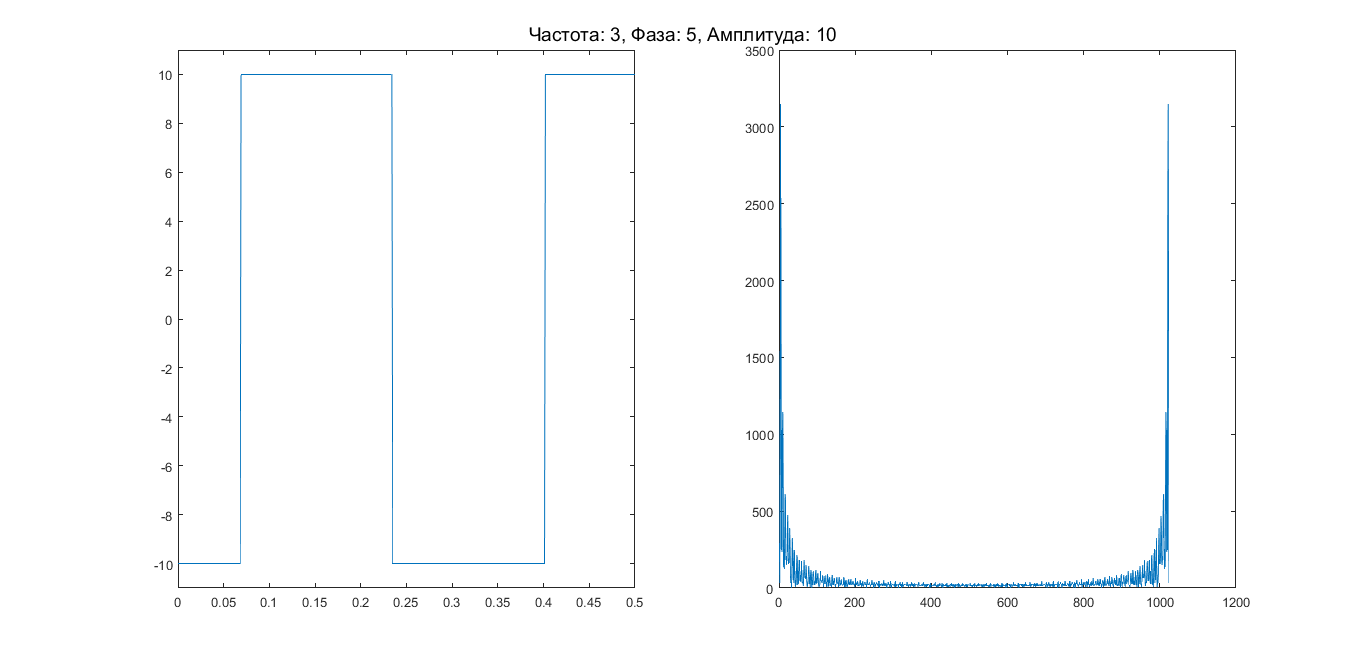
\includegraphics[scale = 0.5]{pictures/3_5_10.png}
	\\ Рис.8 Прямоугольные сигнал и его спектр
	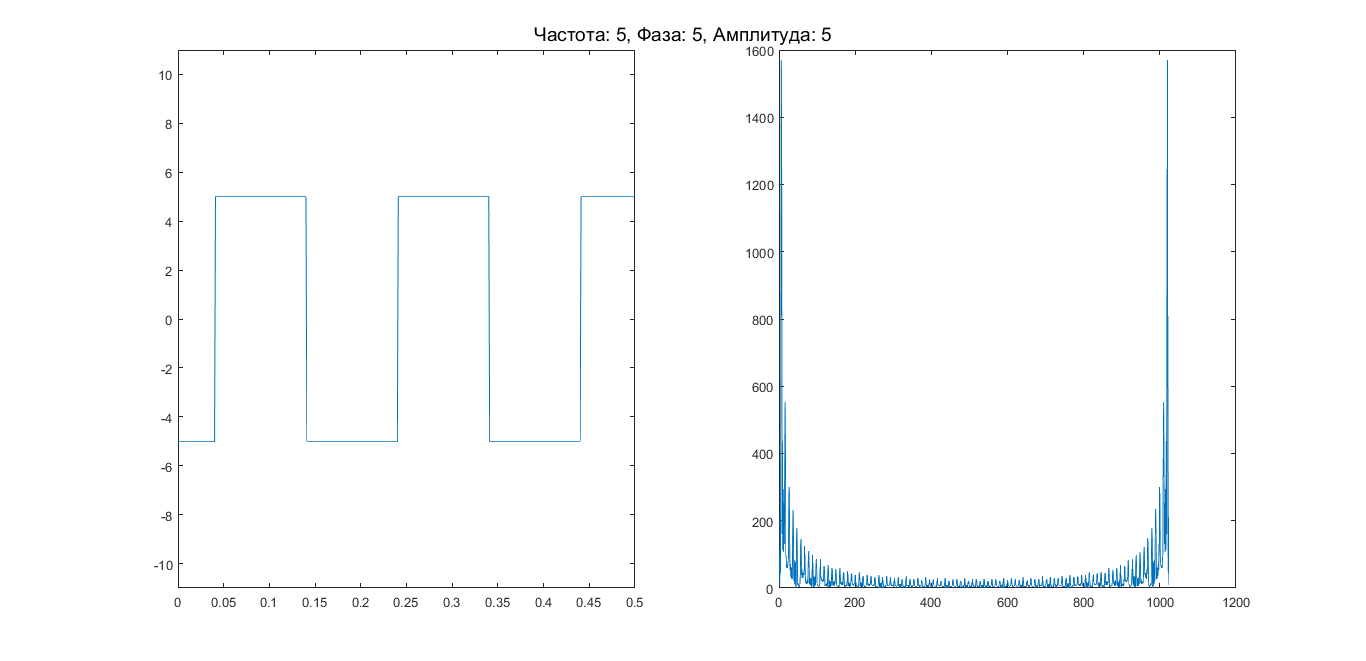
\includegraphics[scale = 0.5]{pictures/5_5_5.png}  
	\\ Рис.9 Прямоугольные сигнал и его спектр
\end{center}

\subsection{Моделирование в Simulink}

В среде Simulink промоделируем синусоидальный сигнал, для этого построим следующую схему.

\begin{center}
	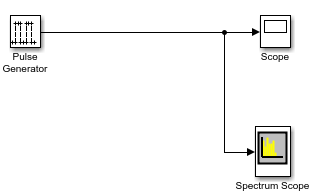
\includegraphics[scale = 0.5]{pictures/prm.png} 
	\\ Рис.10 Схема
\end{center} 
	
В настройках Pulse Generator установим:
\begin{verbatim}
	Amplitude:1
	Period:10
	Pulse width:5
	Phase delay:0
	Sample time:0.01
\end{verbatim}

	\center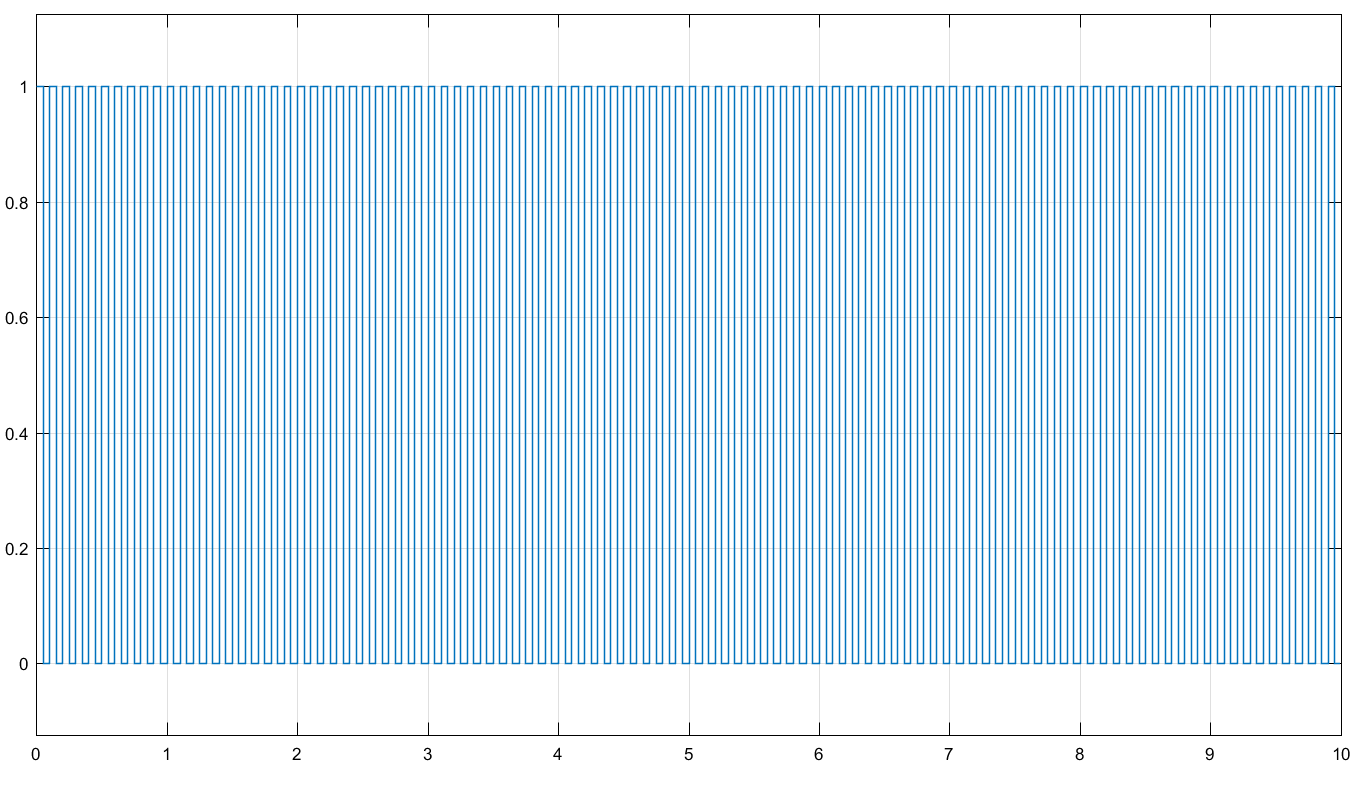
\includegraphics[scale = 0.5]{pictures/simulink.png} 
	\\ \centerРис.11 Сигнал
	\center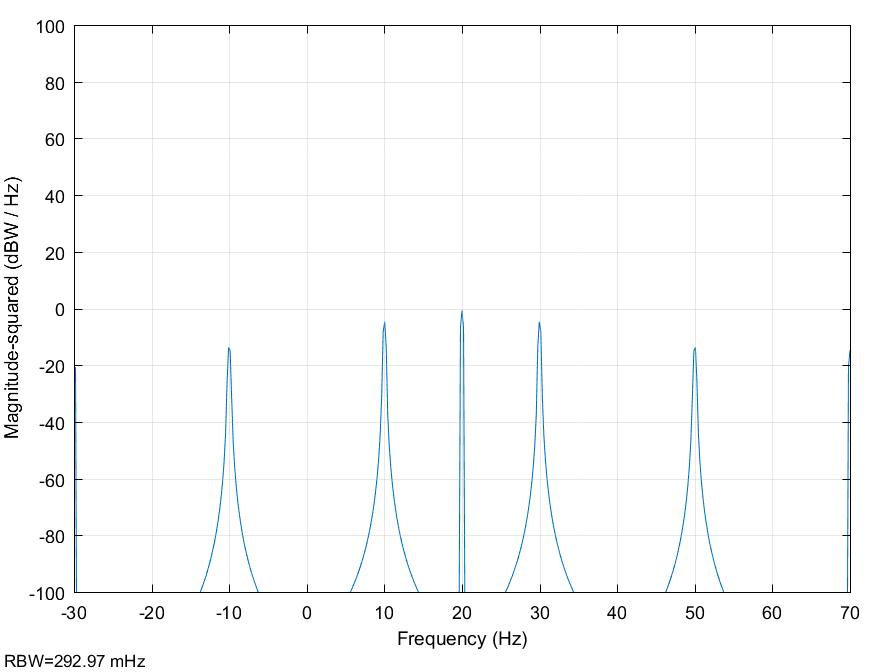
\includegraphics[scale = 0.5]{pictures/simulink_spectr.png} 
	\\ \centerРис.12 Спектр
 
\newpage


\flushleft \section{Выводы}
В ходе выполнения лабораторной работы получены навыки использования средств генерации и визуализации простых сигналов в Matlab и Simulink.\\

Одним из признаков классификации сигналов является способ его задания. Существуют регулярные (детерминированные) и нерегулярные (случайные) сигналы. Детерминированные сигналы задаются аналитической функцией, а случайные принимают произвольные значения в каждый момент времени.\\

Также сигналы классифицируют в зависимости от функций, которые описывают их параметры. Выделяют следующие сигналы:
\begin{itemize}
	\item аналоговые сигналы, описываемые непрерывной функцией;
	\item дискретные сигналы, описываемые функцией взятых в определенные моменты времени отсчетов;
	\item сигналы, квантованные по уровню;
	\item цифровые сигналы (дискретные и квантованные по уровню).
\end{itemize}
\end{document}






